\subsection{The Gaussian fixed point} 
We're now in the position 
to do some actual calculations using 
the renormalisation group flow. 
Our simplest case is, of course, 
the quadratic free energy. Let's consider what happens 
when we have our usual free energy to quadratic order. 
The first thing we do is to expand $ \phi $ in terms 
of Fourier modes, remembering to impose 
the ultraviolet cutoff $ \Lambda $. 
\[
	F _ 0 [ \phi ] = \int d^ d x \left[  \frac{1}{2 } ( \nabla \phi ) ^ 2 + \frac{1}{2 } \mu _ 0 ^ 2 \phi ^ 2 \right] = \int_ 0 ^ \Lambda \frac{ d^ d k }{ ( 2 \pi ) ^ d } \frac{1}{2 } \left(  k ^ 2 + \mu_ 0 ^ 2   \right)  \phi 
	_{ \vec{k} } \phi _{ - \vec{k}}
\] The useful thing about having 
a quadratic free energy like this 
is that this separates into low and high 
Fourier modes with 
\[
	F _ 0 [ \phi ] = F_0 [ \phi ^ - ] + F _ 0 [ \phi ^ + ] 
\] You can prove this yourself 
by simply decomposing
\[
 \phi _{ \vec{k} } = \phi_{ \vec{k} } ^ + + \phi _{ \vec{k} } ^ - 
\]   
When we integrate over, the mixed terms go to zero since
there is no portion of the integral where both the high 
frequency and low frequency modes are non-zero. 
This means that when we write out 
our effective free energy, we get that 
\begin{align*}
e ^{  - F ' [ \phi ^ - ] } &= \left[  \int \mathcal{ D } \phi ^+ e ^{  - F _ 0 [ \phi ^ +  ] }\right] e^{  - F_0 [ \phi ^ -  ] }    \\
			   &=  \mathcal{ N } e ^{  - F_ 0 [ \phi ^ - ] } 
\end{align*} We don't
care about the constant $ \mathcal{ N } $ since it 
doesn't change the physics. The upshot 
of this is that now we have an expression for 
our effective free energy in terms of low frequency modes
$ \phi _{ \vec{k} } ^ - $. 
\[
F' [ \phi ^ - ] = \int ^ \frac{ \Lambda }{ \zeta } 
\frac{ d ^ d k  }{ ( 2 \pi ) ^ d   } \frac{1}{2 } 
( k ^ 2 + \mu _ 0 ^ 2 ) \phi _{ \vec{k} } ^ - \phi _{ -\vec{k} } ^ - 
\]  Now that we've performed the cut-off 
procedure, we need to wrangle the upper bound of the integral 
into its original form. This is done by rescaling 
our Fourier mode variable through 
\[
k ' = k\zeta , \phi'_{ \vec{k} ' } =  \zeta^{ - w } \phi _{\vec{k} } ^ -   \implies 
F' [ \phi ' ] = \int ^ \Lambda \frac{ d ^ d k ' }{ ( 2 \pi ) ^ d } 
\zeta ^{ - d  } \frac{1}{2 } ( \zeta ^{ -2 } ( k ')  ^ 2  + \mu _ 0 ^ 2 ) 
\zeta ^{ 2 w } \phi_{\vec{k} ' } ' \phi _{  - \vec{k}  ' } ' 
\] Now, the aim of the game is to 'canonically normalise' 
our first term $ ( k ' ) ^2  $ since its associated with 
our kinetic gradient in our free energy (and hence should not be 
changed under RG group flow. This is achieved by solving
for our scaling parameter $ w $ and setting it to 
$ w = \frac{ d + 2 }{ 2 }$. This gives our final free energy as
\[
	F _ 0 [ \phi ' ] = 
	\int \frac{ d ^ d k  }{( 2 \pi ) ^ d  } 
	\frac{1}{2 } ( k ^ 2  + \zeta ^ 2 \mu _ 0 ^ 2 ) \phi _{ \vec{k} } \phi _{  - \vec{k} } 
\]  Now, we're in business because we 
can just read off the coupling constant and
we find that $ \mu ^ @ $  oru
coupling parameter scales like 
\[
 \mu ^ 2 ( \zeta ) = \zeta ^ 2 \mu ^ 2 _ 0 
\] Once we have this, we can find 
our fixed points which satisfy the relation 
$ \frac{ d \mu ^ 2  }{ d  \zeta} =0  $. Hence, we 
have that 
\[
 \mu ^ 2 = \infty, \quad \mu ^ 2 = 0  
\] are our fixed points!
Our point $ \mu ^ 2  = 0 $ is called our Gaussian 
fixed point. Right now, these
points are uninteresting, but let's go along with it. 
We add an infinite series of coupling constants, much 
like a Taylor expansion. Then,
we'll look at the behaviour of these coupling 
constants near the point $ \mu _ 0 ^ 2 = 0 $. 


\subsubsection{Expanding around the Gaussian fixed point}
Moving on from our expression above,
let's generalise this further by expanding 
in higher orders of $ \phi $. 
We expand our free energy in a power series as
 \[
	 F [ \phi ]  = \int d ^ d x \left[ \frac{1}{2 } ( \nabla \phi ) ^ 2 + 
	 \frac{1}{2 } \mu ^ 2 _ 0 \phi ^ 2 + \sum_{ n = 4 } g_{ 0 , n } \phi ^ n \right]  
\]  Having these
extra terms mean that when we decompose our 
Fourier modes into low frequency and 
high frequency modes, we have that 
the coupling constants shift when we integrate them out. 
We'll offer a more detailed explanation in 
specifically calculating these shifts, but just for now, 
lets assume that we have that 
\[
 g _{ 0 , n } \to g_{ n } ' = g _{ 0 , n } + \delta g _{ n }
\] We're in good shape to now 
perform RG flow on this free energy. To do RG flow, 
this time in position space, we use the scaling arguments 
we used earlier to determine critical exponents. 
Since we're working in negative scaling dimension, 
we set that 
\[
 \vec{x} \to \vec{x} ' = \vec{x}/\zeta, \quad 
 \phi( \vec{x} ) \to \phi ' ( \vec{x} ' )  = \zeta ^{ \Delta_ \phi  }
 \phi ( \vec{x} ) 
\] Again, as before, we have that 
$ \Delta _{ \phi } $ is a scaling 
dimension to determine. 
Inverting these expressions and substituting them into the free energy, we have that in terms of rescaled parameters, 
\[
 F [ \phi ] = 
 \int d ^ d x \, \zeta ^{ d } \frac{1}{2 } 
\left(  \zeta ^{ - 2 \Delta \phi - 2 } \nabla \phi \cdot  \nabla \phi + 
\frac{1}{2 } \mu _ 0 ^ 2 \zeta ^{ - 2 \Delta \phi  } \phi ^ 2 + 
\sum_{ n = 4 } ^ \infty \zeta ^{ - n \Delta \phi } \phi ^{ n } \right)  \] One should be careful 
when doing these kinds of calculations. 
First, it's important to remember to appropriately 
scale the Jacobian factor (if not, our dependence 
on dimension which we have so pressingly made a point of 
wouldn't be there in the first place  !). Also, when rescaling 
the gradient terms, we have to be careful to 
also scale the derivatives with the 
RG flow as well. 

Asserting that the gradient term should 
be invariant under our renormalisation gives 
us the relation that 
\[
\Delta _{ \phi } = \frac{ d + 2 }{ 2 }
\] This is great because 
since we've determined what $ \Delta_{ \phi } $
is, we can then substitute this into 
our interaction terms. For our coupling constants, we 
then see that our flow induces a scaling on 
$ g_n $ via 
\[
g _ n ( \zeta ) = \zeta ^{ d - n \Delta \phi } g_{ 0 , n }
\] The upshot of dong this process 
is that now we can see under what conditions 
$ g _ n $ flow towards, or diverge from, 
fixed points. Take the case when $ n = 4 $. 
Our coupling constant then evolves like 
\[
g _ 4 ( \zeta ) = \zeta ^{ d -4  } g_{ 0 , 4 }
\] This means that we can classify 
our deformations around fixed points depending on 
our dimension. So, we have that 
\begin{enumerate}
\item $ d > 4 , \phi ^ 4 $ irrelevant 
\item $ d < 4 , \phi ^ 4 $ Relevant 
\item $ d  = 4, \phi ^ 4 $ Marginal 
\end{enumerate} 
\subsubsection{A remark on 'tuning' to remain at a fixed point}
Let's just think about 
the slice of theory space which includes only 
$ \mu _ 0 ^ 2 $ and $ g _ 4 $. We've shown that 
in any case, when we act on out theory space 
with our renormalisation procedure we have that 
$ \mu _ 0 ^ 2  $ goes away from our fixed point. 
This means to stay at this point, we have to 
'fine tune' $ \mu _ 0 ^ 2 $ to stay there. 
However, depending on our 
critical dimension $ d =  4 $, 
we can either fine tune $ g _ 4 $ if 
our deformation is relevant ( d < 4 ) or not care about it
when it's irrelevant ( d > 4 ) with the confidence that 
it'll return back to the fixed point.

In the figure below we have a diagram to show this 
behaviour. 

\begin{figure}[htpb]
	\centering
	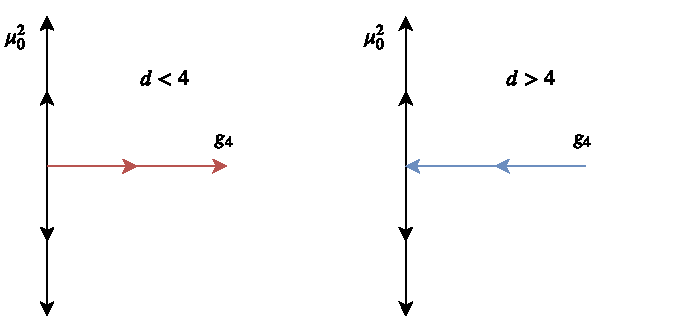
\includegraphics[width=0.8\linewidth]{figures/rg_flow.pdf}
	\caption{}%
	\label{fig:}
\end{figure}

\subsubsection{$ \mathbb{ Z} _ 2 $ Symmetry breaking } 
Typically, we have that RG flow doesn't break our 
symmetries. This symmetry is respected by momentum, 
so in momentum space symmetry is also preserved. This means 
that every term in our decomposition 
\[
 F_ 0 [ \phi ] = F_ 0 [ \phi ^ - ]  + F_0 [ \phi ^ + ] + F_I [ \phi ^ - , \phi ^ + ] 
\] At low temperature, 
our background magnetic field, becomes important. 
We need to have an RG way of visualising what's going on. 


\pagebreak 
